\documentclass[11pt,a4paper]{article}

\usepackage[utf8]{inputenc}
\usepackage[T1]{fontenc}
\usepackage[french]{babel}
\usepackage[a4paper,margin=2.3cm]{geometry}
\usepackage{graphicx}
\usepackage{booktabs}
\usepackage{float}
\usepackage{caption}
\usepackage{xcolor}
\usepackage[hidelinks]{hyperref}

% Cherche les figures dans plusieurs emplacements (local report/, ou Overleaf)
\graphicspath{{../figures/}{figures/}{./}}
\captionsetup{font=small,labelfont=bf}

% Marqueur pour les passages a personnaliser par l'equipe
\newcommand{\ajuster}[1]{\textcolor{red}{[\textbf{A AJUSTER} : #1]}}

\title{\vspace{-1.5cm}\textbf{Peut-on prédire le succès d'une expédition himalayenne~?}\\[0.3cm]
\large Introduction au Traitement des Données --- Projet Kaggle}
\author{Romain Ben \and Loriziano Soave \\[0.2cm]
\small Polytech Nice Sophia, MAM3 --- Lionel Fillatre, 2025-2026}
\date{}

\begin{document}
\maketitle
\vspace{-0.8cm}

% =====================================================================
\section{Business goal}
% =====================================================================

Chaque année, des centaines d'expéditions tentent de gravir les sommets de
l'Himalaya. Toutes ne réussissent pas. Notre question est la suivante~:

\begin{quote}
\itshape Peut-on prédire si une expédition himalayenne atteindra le sommet,
à partir des seules informations connues \textbf{avant le départ}~?
\end{quote}

L'enjeu pratique est réel~: une agence d'expédition, un assureur ou un chef
de cordée voudraient estimer leurs chances en amont, lorsqu'il est encore
possible d'ajuster l'équipe, le matériel ou la stratégie. C'est un problème
de \textbf{classification binaire} (succès / échec), que nous traitons par
\textbf{régression logistique}.

\paragraph{Le jeu de données.} Nous utilisons le jeu de données
\textit{Himalayan Expeditions} (Kaggle), issu de la base historique
d'Elizabeth Hawley. Il recense \textbf{11~425 expéditions} décrites par
65~variables. La cible \texttt{success} est presque équilibrée~:
\textbf{55~\% de succès} contre 45~\% d'échec. Cet équilibre est précieux~:
la régression logistique pourra être entraînée sans rééquilibrage, et
l'\textit{accuracy} restera une métrique honnête (un modèle naïf qui
prédirait toujours «~succès~» n'atteindrait que 55~\%).

\paragraph{Une contrainte centrale~: éviter le \textit{data leakage}.} Notre
question impose une discipline. De nombreuses variables du jeu de données
décrivent ce qui s'est passé \textbf{pendant} ou \textbf{après} l'expédition
(nombre de membres ayant atteint le sommet, décès, date de sommet, durée
totale). Les utiliser reviendrait à «~prédire le résultat avec le
résultat~». Nous les avons donc systématiquement écartées des prédicteurs~:
\texttt{smtmembers}, \texttt{mdeaths}, \texttt{smthired}, \texttt{hdeaths},
\texttt{smtdate}, \texttt{termdate}, \texttt{totdays}.

\paragraph{Point de départ assumé.} Le règlement autorise à s'appuyer sur les
contributions publiées. Nous partons donc de la vingtaine de variables
retenues par Muhammed Ali Yilmaz dans son notebook Kaggle, plutôt que des
65~colonnes brutes. Notre travail de nettoyage et de sélection s'effectue sur
cette base déjà dégrossie, ce qui nous permet de concentrer l'effort sur
l'analyse plutôt que sur le tri initial.

% =====================================================================
\section{Team management}
% =====================================================================

Le projet a été mené en binôme par Romain Ben et Loriziano Soave.

\paragraph{Outils.} Nous avons travaillé en \textbf{Python} (pandas, numpy,
matplotlib, seaborn, scikit-learn), organisés en scripts \texttt{.py}
numérotés correspondant aux étapes du pipeline (exploration, wrangling,
visualisation, feature engineering, régression). Le code et les données sont
versionnés sur \textbf{GitHub}~: \url{https://github.com/BnRomain/Introduction_TraitementDonnees}.

\paragraph{Méthode de collaboration.} Nous avons adopté un flux de travail
git sur une branche unique, avec synchronisation fréquente
(\texttt{pull -{}-rebase}) avant chaque contribution pour limiter les
conflits. Chaque décision importante (choix d'une variable, rejet d'une
feature) est documentée directement en commentaire dans le code, afin que les
deux membres partagent le même raisonnement.

\paragraph{Répartition du travail.}
\ajuster{décrire qui a fait quoi, par exemple~: Romain sur l'exploration et
le wrangling, Loriziano sur la visualisation et le feature engineering,
régression et rapport en commun. Adapter à la réalité.}

\paragraph{Démarche.} Notre fil conducteur a été de ne jamais retenir une
variable «~au feeling~». Chaque choix s'appuie sur une preuve chiffrée tirée
des données, et nous avons accepté de \textbf{rejeter} nos propres
hypothèses lorsque les données les contredisaient (voir
section~\ref{sec:features}). Cette honnêteté est, selon nous, le c\oe ur de
la démarche scientifique.

% =====================================================================
\section{Visualisation des données}
% =====================================================================

Avant de modéliser, nous cherchons à \textbf{comprendre les relations} entre
les variables et le succès. Notre méthode repose sur deux outils
complémentaires.

\paragraph{Outil 1~: le croisement variable~/ cible.} En groupant les
expéditions par une variable et en calculant le taux de succès moyen
(\texttt{groupby().mean()}), on révèle immédiatement un signal. C'est ainsi
que l'oxygène est apparu comme le facteur le plus déterminant
(figure~\ref{fig:o2})~: le taux de succès \textbf{passe de 45~\% à 80~\%}
selon que l'expédition utilise ou non de l'oxygène en bouteille.

\begin{figure}[H]
\centering
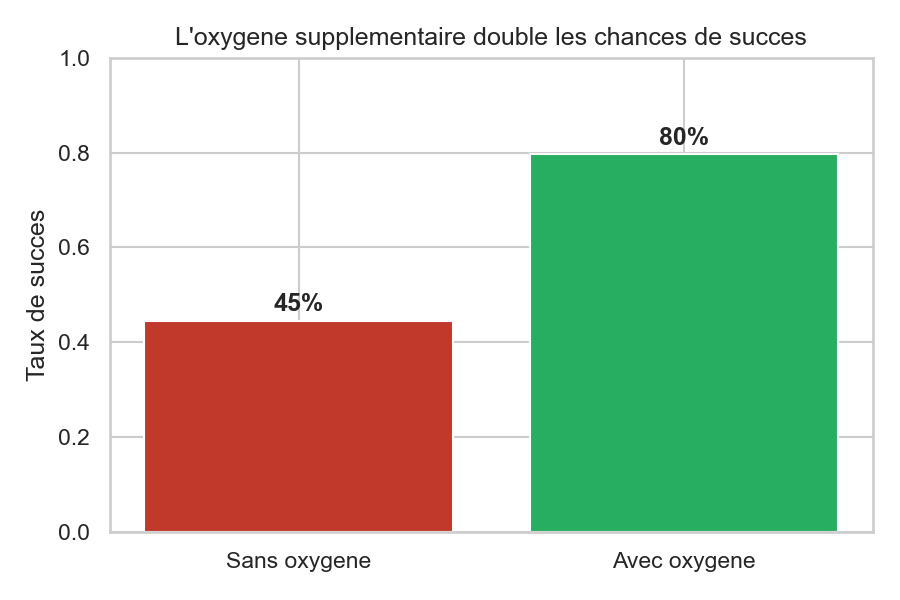
\includegraphics[width=0.55\textwidth]{01_effet_oxygene.png}
\caption{L'oxygène supplémentaire double presque les chances de succès.
C'est le signal le plus fort du jeu de données.}
\label{fig:o2}
\end{figure}

\paragraph{Outil 2~: la matrice de corrélation.} La heatmap
(figure~\ref{fig:corr}) donne la vue d'ensemble des liens \textit{linéaires}
entre variables numériques. Elle sert deux objectifs~: repérer ce qui corrèle
avec la cible (\texttt{o2used}~: 0{,}32~; \texttt{camps}~: 0{,}28~;
\texttt{comrte}~: 0{,}22), et détecter les \textbf{redondances}. On y voit
notamment que \texttt{tothired} et \texttt{totmembers} sont corrélées
(0{,}58)~: les grosses équipes embauchent plus de Sherpas. Cette redondance
nous a directement inspiré une feature (section~\ref{sec:features}).

\begin{figure}[H]
\centering
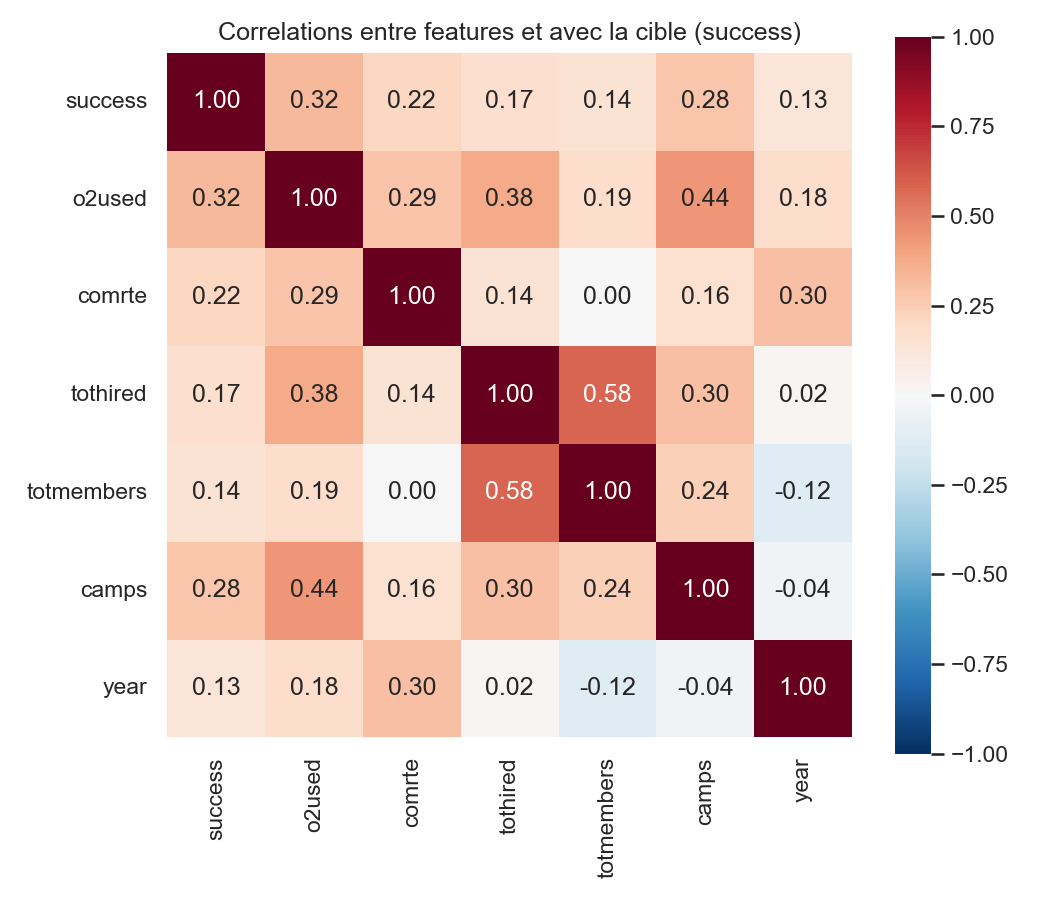
\includegraphics[width=0.62\textwidth]{04_correlations.png}
\caption{Corrélations entre prédicteurs et avec la cible. Outil de vue
d'ensemble, limité aux variables numériques et aux liens linéaires.}
\label{fig:corr}
\end{figure}

\paragraph{Croiser deux variables~: la heatmap 2D.} Pour aller plus loin que
les corrélations, nous croisons deux variables contre la cible. La
figure~\ref{fig:sherpas} montre le taux de succès selon la taille de l'équipe
(colonnes) et le nombre de Sherpas (lignes). La lecture est éloquente~: en
parcourant une colonne de bas en haut (équipe de taille fixée), le succès
\textbf{augmente nettement avec le nombre de Sherpas}, tandis que les lignes
restent assez plates. Ce n'est donc pas la taille brute de l'équipe qui
compte, mais la \textit{proportion} de personnel d'encadrement.

\begin{figure}[H]
\centering
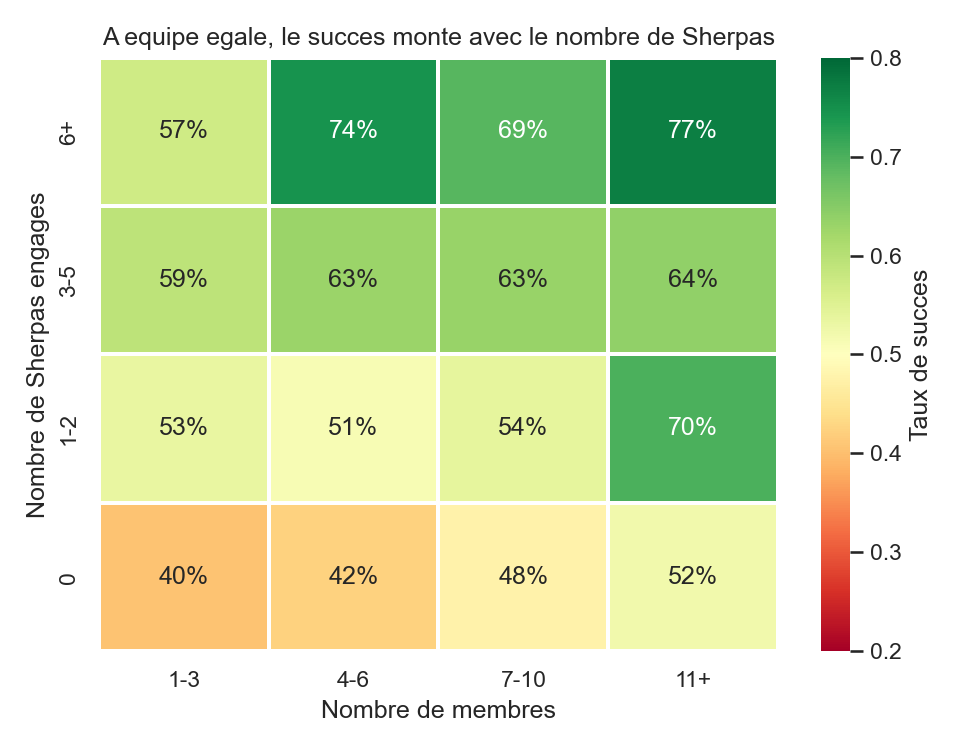
\includegraphics[width=0.62\textwidth]{03_sherpas_vs_membres.png}
\caption{À taille d'équipe égale, le succès monte avec le nombre de Sherpas.
Les cases reposant sur moins de 20 expéditions sont masquées pour ne pas
tirer de conclusion sur de trop petits effectifs.}
\label{fig:sherpas}
\end{figure}

% =====================================================================
\section{Handcrafted features}
\label{sec:features}
% =====================================================================

Cette section illustre notre démarche~: pour chaque feature inventée, nous
formulons une hypothèse, nous la testons sur les données, puis nous décidons
de la garder ou non. Sur trois features bricolées, \textbf{une seule a
survécu}, et c'est précisément ce qui rend la démarche crédible.

\subsection*{A. \texttt{ratio\_hired}~: la proportion de Sherpas (GARDÉE)}

\textbf{Hypothèse.} Suite à la figure~\ref{fig:sherpas}, ce n'est pas le
nombre brut de Sherpas qui compte mais leur proportion. Nous définissons
\texttt{ratio\_hired} $=$ \texttt{tothired} $/$ \texttt{totmembers}.

\textbf{Test.} Le taux de succès croît de façon nette avec le ratio
(figure~\ref{fig:ratio})~: \textbf{49~\%} pour un ratio inférieur à 0{,}5,
contre \textbf{64~\%} pour un ratio entre 0{,}5 et 1. \textbf{Décision~:
gardée.}

\begin{figure}[H]
\centering
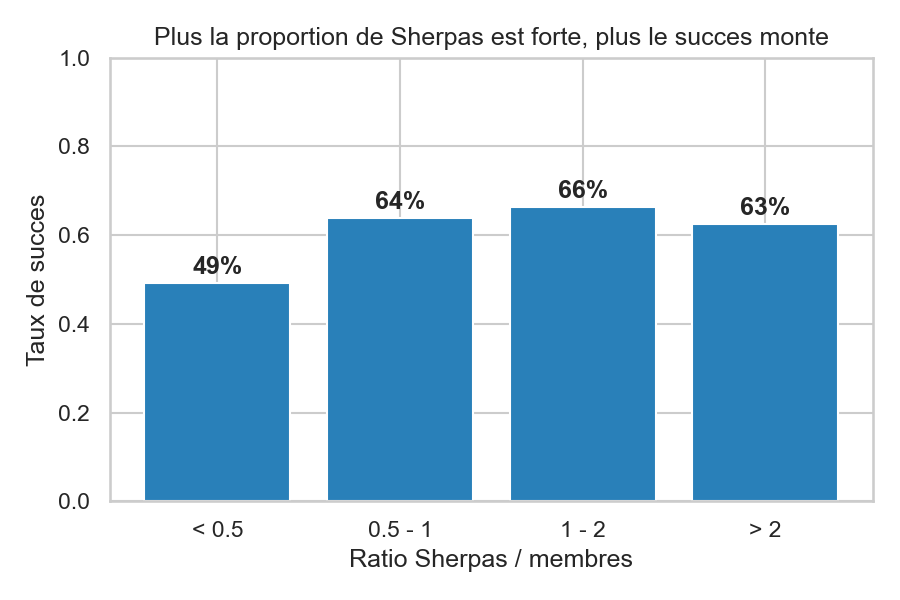
\includegraphics[width=0.5\textwidth]{05_ratio_hired.png}
\caption{Plus la proportion de Sherpas par membre est élevée, plus le taux
de succès augmente.}
\label{fig:ratio}
\end{figure}

\subsection*{B. \texttt{o2used} $\times$ \texttt{season}~: une fausse
interaction (REJETÉE)}

\textbf{Hypothèse.} La figure~\ref{fig:interaction} semblait montrer que
l'effet de l'oxygène \textit{dépend} de la saison~: $+46$ points au
printemps, quasi nul en hiver. Cela suggérait une interaction à encoder.

\textbf{Test critique.} Deux objections nous ont alertés. D'abord les
\textbf{effectifs}~: seulement 40~expéditions «~hiver $+$ O\textsubscript{2}~»
et 9~«~été $+$ O\textsubscript{2}~», trop peu pour conclure. Ensuite la
\textbf{physique}~: l'oxygène aide partout en altitude, la saison ne change
pas la pression partielle d'O\textsubscript{2}. Nous avons donc cherché une
\textbf{variable confondante}, et nous l'avons trouvée~: l'oxygène est
concentré sur l'Everest (76~\% des expéditions Everest), et l'Everest se
tente à 88~\% au printemps. Résultat~: la catégorie «~printemps $+$
O\textsubscript{2}~» est en réalité composée à 68~\% d'expéditions Everest.
Ce n'est pas la saison qui module l'effet de l'oxygène, c'est le
\textbf{sommet tenté}. \textbf{Décision~: rejetée} (corrélation n'est pas
causalité).

\begin{figure}[H]
\centering
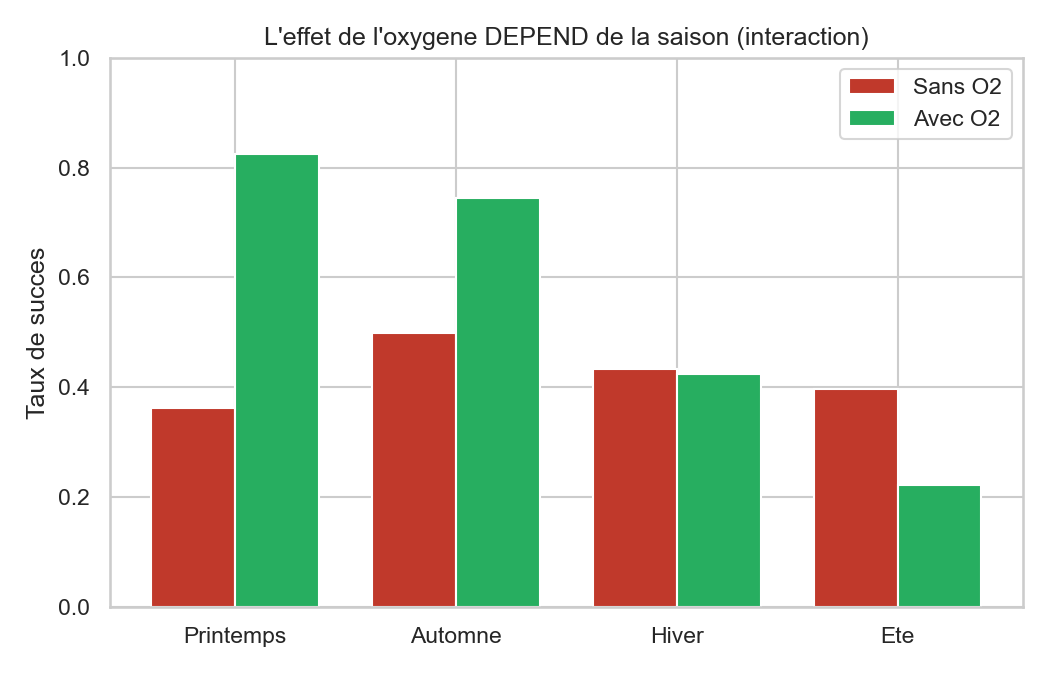
\includegraphics[width=0.6\textwidth]{02_interaction_o2_saison.png}
\caption{L'apparente «~interaction~» oxygène $\times$ saison. Le signal est
un artefact~: la saison est corrélée au sommet tenté, qui porte la vraie
explication.}
\label{fig:interaction}
\end{figure}

\subsection*{C. \texttt{rope\_bool}~: usage de corde fixe (REJETÉE)}

\textbf{Hypothèse.} La variable \texttt{rope} (longueur de corde fixe, en
mètres) comporte 84~\% de zéros. Nous l'avons transformée en booléen
«~corde utilisée ou non~», pensant qu'une expédition mieux préparée poserait
de la corde.

\textbf{Test.} Les données réfutent l'hypothèse~: \textbf{55~\% de succès
sans corde contre 54~\% avec} (figure~\ref{fig:rope}), un écart nul, voire
inversé. De plus, la corde est posée \textit{pendant} l'ascension (risque de
\textit{leakage}) et les 84~\% de zéros traduisent sans doute une donnée non
renseignée. \textbf{Décision~: rejetée.}

\begin{figure}[H]
\centering
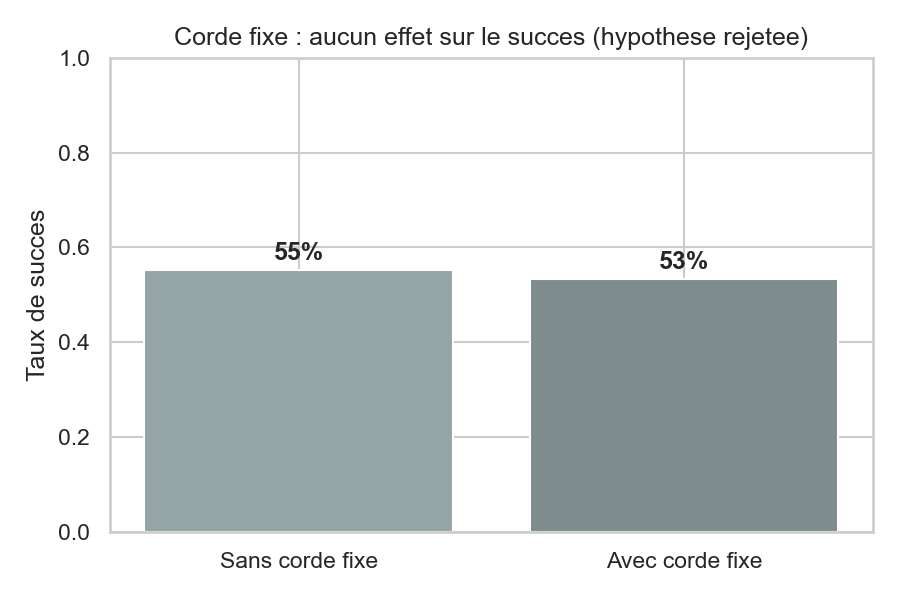
\includegraphics[width=0.5\textwidth]{06_rope_bool.png}
\caption{L'hypothèse «~corde fixe = plus de succès~» n'est pas vérifiée par
les données. Une hypothèse testée et rejetée fait partie d'une analyse
honnête.}
\label{fig:rope}
\end{figure}

% =====================================================================
\section{Régression logistique}
% =====================================================================

\paragraph{Variables finales.} Après nettoyage (suppression de 2~saisons
«~Unknown~» et de 63~expéditions sans membre), le jeu de données propre
compte \textbf{11~362~expéditions}. Les prédicteurs sont~: \texttt{o2used},
\texttt{comrte}, \texttt{tothired}, \texttt{totmembers}, \texttt{camps},
\texttt{year}, \texttt{ratio\_hired}, ainsi que \texttt{season} et
\texttt{peakid} (regroupé aux 8~sommets les plus tentés $+$ «~Autre~»)
encodés en \textit{one-hot}.

\paragraph{Pipeline.} (1)~Séparation $X$ / $y$~; (2)~découpage train/test
80/20~; (3)~\textbf{standardisation des variables numériques calée sur le
train uniquement} (pour éviter que le test ne fuite dans la moyenne et
l'écart-type)~; (4)~entraînement de \texttt{LogisticRegression}~;
(5)~évaluation sur le test (accuracy, précision, rappel, matrice de
confusion, ROC-AUC).

\paragraph{Le test du \textit{data leakage} sur \texttt{camps}.} Notre
analyse a révélé que \texttt{camps} (nombre de camps installés) contient une
fuite~: sur l'Everest, le taux de succès saute de 22~\% (2~camps) à 71~\%
(3~camps), car l'assaut final part du camp~4. La variable mesure donc en
partie «~jusqu'où l'expédition est montée~», ce qui est presque le résultat.
Nous entraînons donc \textbf{deux modèles, avec et sans \texttt{camps}}, pour
mesurer concrètement l'ampleur de cette fuite.

\begin{table}[H]
\centering
\caption{Performances des modèles sur le jeu de test (à compléter après
exécution de \texttt{05\_regression.py}).}
\begin{tabular}{lccc}
\toprule
Modèle & Accuracy & ROC-AUC & Écart au \textit{baseline} (55~\%) \\
\midrule
Baseline (classe majoritaire) & 0{,}55 & --- & --- \\
Régression logistique (sans \texttt{camps}) & \ajuster{} & \ajuster{} & \ajuster{} \\
Régression logistique (avec \texttt{camps}) & \ajuster{} & \ajuster{} & \ajuster{} \\
\bottomrule
\end{tabular}
\end{table}

\paragraph{Interprétation des coefficients.} \ajuster{commenter les
coefficients une fois le modèle entraîné. Pistes attendues~: signe positif
fort pour \texttt{o2used} et \texttt{ratio\_hired}~; les coefficients
\texttt{peakid} s'interprètent par rapport au sommet de référence
(AmaDablam)~; un coefficient \texttt{peakid\_EVER} positif signifierait
«~plus de chances de succès que l'AmaDablam~», ce qui sera à confronter à
notre intuition.} Nous vérifierons enfin l'absence de sur-apprentissage en
comparant les performances sur le train et sur le test.

% =====================================================================
\section{Conclusion}
% =====================================================================

Notre analyse dégage une hiérarchie claire des facteurs de succès d'une
expédition himalayenne. L'\textbf{usage de l'oxygène} domine, suivi de
l'\textbf{encadrement} (route commerciale, proportion de Sherpas) et de la
\textbf{difficulté intrinsèque du sommet}. Ces résultats sont cohérents avec
le bon sens alpin, ce qui crédibilise l'approche.

Au-delà des chiffres, le projet illustre deux pièges classiques du traitement
de données que nous avons su identifier. Le \textbf{data leakage}~: certaines
variables séduisantes (\texttt{camps}) contiennent en réalité le résultat.
La \textbf{confusion entre corrélation et causalité}~: notre «~interaction~»
oxygène $\times$ saison n'était qu'un reflet du sommet tenté. Dans les deux
cas, ce sont le raisonnement métier et le test critique, plus que les
statistiques brutes, qui ont permis de trancher.

\paragraph{Limites et pistes.} La qualité des données reste inégale (zéros
ambigus, dates manquantes). Une amélioration naturelle serait d'intégrer
l'\textbf{altitude du sommet} comme variable continue (plutôt que
\texttt{peakid} en one-hot), qui résumerait mieux la difficulté. On pourrait
aussi comparer la régression logistique à un modèle non linéaire pour vérifier
si des interactions plus fines existent, tout en restant vigilant sur le
\textit{leakage}.

% =====================================================================
\section{Références}
% =====================================================================

\begin{enumerate}\itemsep0pt
\item Jeu de données~: \textit{Himalayan Expeditions}, Kaggle.
\url{https://www.kaggle.com/datasets/siddharth0935/himalayan-expeditions}
\item Notebook d'inspiration~: M.~A.~Yilmaz, \textit{Himalayan Climb
Prediction with ML/DL}, Kaggle.
\url{https://www.kaggle.com/code/muhammedaliyilmazz/himalayan-climb-prediction-with-ml-dl}
\item Source historique~: The Himalayan Database (E.~Hawley).
\item \textit{scikit-learn}~: documentation de \texttt{LogisticRegression}.
\item Dépôt du projet~:
\url{https://github.com/BnRomain/Introduction_TraitementDonnees}
\end{enumerate}

\end{document}
